\documentclass[11pt]{article}

% Template-agnostic preamble — works without any venue style file.
% For venue submission, replace \usepackage[margin=1in]{geometry} with
% e.g. \usepackage{neurips_2024} or \usepackage[accepted]{icml2024}.
\usepackage[margin=1in]{geometry}

\usepackage[utf8]{inputenc}
\usepackage[T1]{fontenc}
\usepackage{hyperref}
\hypersetup{colorlinks=true, linkcolor=blue, citecolor=blue, urlcolor=blue}
\usepackage{url}
\usepackage{booktabs}
\usepackage{amsfonts}
\usepackage{nicefrac}
% \usepackage{microtype}  % requires scalable fonts
\usepackage{xcolor}
\usepackage{graphicx}
\usepackage{caption}
\usepackage{subcaption}
\usepackage{amsmath}
\usepackage{amssymb}
\usepackage{tabularx}
\usepackage{array}
\usepackage{multirow}

\title{Tool-Entropy Collapse: A Cross-Architecture Signature of Agent WANDERING Failure}

\author{%
  Caio Vicentino \\
  OpenInterpretability \\
  Fortaleza, Brazil \\
  ORCID: 0009-0003-4331-6259 \\
  \texttt{caio@openinterp.org}%
}

\begin{document}

\maketitle

\begin{abstract}
Probe-based safety monitoring of LLM agents typically assumes a probe trained to predict trajectory success/failure provides a reliable signal at any turn. We test this on 99 trajectories of Qwen3.6-27B running SWE-bench Pro across 3 codebases and identify two mechanistically distinct sub-classes of agent failure: \textbf{LOCKED} (66\%) and \textbf{WANDERING} (34\%). Both are externally identical---they exhaust the turn budget without emitting \texttt{finish\_tool}---but differ fundamentally in internal state. LOCKED agents are uncertain (probe collapses to $<0.30$ by mean fraction $0.92$ of trajectory length, 21\% never produce a patch). WANDERING agents are over-confident (probe stays $>0.70$ with median final score $1.000$, 95\% produce patches). The 34\% probe-vs-outcome disagreement constitutes a quantified blind spot for probe-only monitoring schemes (bootstrap 95\% CI: $[22.0\%, 45.8\%]$).

We test \textbf{six detector designs across three signal channels} (text, residual cross-layer, action entropy): (v1) post-hoc text monitor---35\% WANDERING recall, 0\% false-positive cost; (v2) naive early-warning text extension---15\% SUCCESS FP, unacceptable; (v3) persistence hypothesis---\emph{empirically refuted in opposite direction} (SUCCESS agents persist longer in completion verbalization, one-tail $p = 0.92$); (v4) cross-layer probe disagreement across L11/23/31/43/55---succeeds (late-half range W vs S $p = 0.0028$, 65\% recall $\times$ 30\% FP $\times$ 15-turn lead); \textbf{(v5) tool-use entropy collapse---55\% recall $\times$ 5\% FP, the breakthrough signal} (Mann-Whitney $p = 1.0\times10^{-6}$, W/S median ratio $0.41$); (v6) residual stability---marginal, dominated by v5. Combined v1 $\cup$ v4 closes 80\% of the blind spot at advisory tier; combined v1 $\cup$ v5 closes \textbf{70\% at Tier-3 autonomous-termination precision (5\% FP)}.

Mid-layer ablation reveals the discrimination is \textbf{edge-layer-driven}: L23/L31/L43 agree, but L11 (surface processing) and L55 (output planning) disagree with the mid-layer consensus more in WANDERING than in SUCCESS. We reframe WANDERING from ``stuck-in-verification-loop'' to ``mid-layer-to-edge-layer alignment failure''.

\textbf{Cross-architecture validation within SWE-bench}: Llama-70b ($n=2{,}315$, $p<10^{-15}$, ratio $0.41$ identical to Qwen) and GPT-5 router ($n=1{,}419$, $p=8.9\times10^{-35}$, ratio $0.71$). Tier 3 holds on Llama: 71\% recall $\times$ 4.1\% FP. \textbf{Cross-task validation on METR MALT (15+ task families, $n=9$ \texttt{gives\_up} $\ne$ behavioral WANDERING) is NULL ($p=0.81$), scoping the claim}: tool-entropy collapse is a robust signature for \emph{multi-turn code-execution agent tasks with rich action spaces}, NOT universally task-invariant. Deployment guidance covers three operational tiers (forensics, advisory escalation, autonomous termination), all shippable.
\end{abstract}

\section{Problem}

Production safety pipelines for LLM agents rely on activation probes as monitoring signals. A common assumption is that probe $=$ trustworthy outcome predictor at any turn. We test this on agent trajectories that fail.

\section{Related work and our position}

\textbf{Probe-based agent monitoring.} Apollo Research \cite{apollo_deception_2025} use linear probes on residual activations to detect strategic deception with AUROC $0.96$--$0.999$. Anthropic's ``Simple probes catch sleeper agents'' \cite{anthropic_sleeper_2024} demonstrates defection probes work across middle layers. Lugoloobi et al. \cite{lugoloobi_2026} predict policy-specific success from pre-generation activations on math/coding. Our work extends this paradigm with three differentiations: (a) we identify a 34\% \emph{blind spot} of probe-based monitoring (the WANDERING sub-class), (b) we use \emph{cross-layer disagreement} (not single-layer probe), and (c) we propose \emph{tool-entropy as a probe-free complementary signal}.

\textbf{Cross-layer probe ensembling.} \cite{multilayer_ensemble_2026} shows multi-layer probe ensembling improves accuracy and robustness---our \S\ref{sec:v4} builds directly on this for WANDERING discrimination via late-half disagreement.

\textbf{Tool-use entropy.} The closest prior art \cite{entropy_tool_use_2026} uses entropy as a \emph{reward signal for RL training} to shape tool-use policies (entropy reduction $\rightarrow$ 72\% fewer tool calls, 22\% performance gain). Our work uses tool-entropy as a \emph{diagnostic signal for failure detection at inference time}, not for training. Same metric, orthogonal direction. \cite{aepo_2025} also uses entropy in agentic RL.

\textbf{Agent failure mode taxonomies.} \cite{mast_2025} identifies 14 multi-agent failure modes with 41--86.7\% production failure rates. \cite{jetbrains_2025} (whose dataset we use in \S\ref{sec:cross-arch}) shows failed SWE-agent trajectories are longer with higher variance---our WANDERING is a specific sub-type that survives turn-length stratification. METR's MALT dataset \cite{malt_2025} contains 32 ``giving up'' examples (which we test in \S\ref{sec:malt})---semantically distinct from our behavioral WANDERING.

\textbf{Trajectory-level failure mechanisms.} \cite{canonical_path_2026} proposes Canonical Path Deviation as a causal mechanism of agent failure. \cite{elpo_2026} localizes first-irrecoverable-step via binary-search rollouts. Our inflection-turn analysis (\S\ref{sec:results}) provides a rollout-free analog: probe lock-in identifies ``first stable-verdict step'', which occurs \emph{after} the irrecoverability point.

\textbf{SWE-bench.} SWE-bench Pro \cite{swebench_pro_2025} is the benchmark we run on. SWE-agent \cite{swe_agent_2024} is the scaffold framework. SWE-smith \cite{swe_smith_2025} is the dataset corpus used by JetBrains and SWE-bench/SWE-smith-trajectories.

\textbf{Our novel contributions:}
\begin{enumerate}
\item Quantification of the 34\% WANDERING blind spot with bootstrap 95\% CI $[22.0\%, 45.8\%]$
\item Edge-layer-driven cross-layer disagreement as Tier 2 advisory signal (\S\ref{sec:v4-midlayer} mid-layer ablation)
\item Tool-entropy collapse with ratio invariance (W/S $= 0.41$ in Qwen and Llama, $0.71$ in GPT-5) as Tier 3 autonomous-termination signal (\S\ref{sec:v5})
\item 3-tier deployment framework integrating forensics $+$ advisory $+$ autonomous (\S\ref{sec:deployment}, \S\ref{sec:deployment-revised})
\item Cross-architecture validation in SWE-bench (3 labs / 3 scaffolds) $+$ honest scope limit via MALT null (\S\ref{sec:malt})
\end{enumerate}

\section{Setup}

\begin{itemize}
\item \textbf{Model}: Qwen3.6-27B (Alibaba 2026)
\item \textbf{Task}: SWE-bench Pro (Pro-balanced split)
\item \textbf{Dataset}: 99 trajectories from OpenInterp Phase 6 capture, residuals at L11/L23/L31/L43/L55 per turn
\item \textbf{Outcome label}: \texttt{finish\_reason == "finish\_tool"} ($n=40$ success) vs \texttt{"max\_turns"} ($n=59$ failure)
\item \textbf{Probe}: top-10 diff-means features at L43 \texttt{pre\_tool} + StandardScaler + LogisticRegression
\item \textbf{Methodology}: 5-fold cross-validation; probe re-trained on representative residual (mean across all turns) within each fold; per-turn scores computed on held-out trajectories
\end{itemize}

\section{Results}\label{sec:results}

\subsection{Baseline probe performance}
Trajectory-mean residual at L43 \texttt{pre\_tool} achieves CV AUROC $= \mathbf{0.934 \pm 0.041}$.

\subsection{Inflection-turn distribution}
For each trajectory, define \texttt{lock\_fail} as the earliest turn $T$ such that probe\_score$(t) < 0.30$ for all $t \in [T, \text{end}]$ (similarly \texttt{lock\_succ} for $>0.70$).

\begin{table}[h]
\centering
\caption{Lock-in turn distribution across outcome classes.}
\begin{tabular}{lcccc}
\toprule
Class & $n$ & Lock-in rate & Median lock turn & Median fraction of length \\
\midrule
Success & 40 & 100\% & 33 (Q1=25, Q3=38) & \textbf{0.88} \\
Failure (LOCKED) & 39 & --- & 46 (Q1=43, Q3=49) & \textbf{0.92} \\
Failure (WANDERING) & 20 & --- & never reaches fail-lock & --- \\
\bottomrule
\end{tabular}
\end{table}

Two key observations: (1) lock-in happens only in the final $\sim$10\% of trajectory length, and (2) \textbf{34\% of failures never commit to the failure regime}---the WANDERING sub-class.

\subsection{The WANDERING sub-class}
\begin{table}[h]
\centering
\caption{Statistics for the 20 WANDERING failures vs 39 LOCKED failures.}
\begin{tabular}{lccc}
\toprule
Metric & LOCKED & WANDERING & Mann-Whitney $p$ \\
\midrule
Final probe score (median) & 0.000 & \textbf{1.000} & $<0.0001$ \\
First-turn probe score (median) & 1.000 & 1.000 & 0.92 \\
Patch produced (rate) & 79\% & \textbf{95\%} & --- \\
Patch size if any (median bytes) & 4172 & 4065 & --- \\
0.5-crossings & 15 & 18 & 0.35 \\
\bottomrule
\end{tabular}
\end{table}

WANDERING agents end with probe-confident-success, almost always produce a patch, but behaviorally fail.

\subsection{Bootstrap CI on the WANDERING rate}
At L43 \texttt{pre\_tool}, 10,000-sample bootstrap (resampling 59 failure trajectories): point estimate \textbf{33.9\%}, 95\% CI $[22.0\%, 45.8\%]$.

\subsection{Cross-layer robustness}
\begin{table}[h]
\centering
\caption{Per-layer CV AUROC and WANDERING rate.}
\begin{tabular}{lcc}
\toprule
Layer & CV AUROC & WANDERING rate \\
\midrule
L11 & $0.873 \pm 0.094$ & $14/59 = 24\%$ \\
L23 & $0.933 \pm 0.038$ & $19/59 = 32\%$ \\
L31 & $0.928 \pm 0.049$ & $23/59 = 39\%$ \\
\textbf{L43} & $\mathbf{0.934 \pm 0.041}$ & $\mathbf{20/59 = 34\%}$ \\
L55 & $0.888 \pm 0.055$ & $33/59 = 56\%$ \\
\bottomrule
\end{tabular}
\end{table}

\section{Six detector designs}

We test detectors across three signal channels (text, residual cross-layer, action entropy).

\subsection{v1: Post-hoc text monitor (Tier 1 forensics)}
Operationally: \texttt{alarm = probe<0.5 OR (completion\_phrase\_in\_last5 AND no\_finish AND patch>0)}. Result: \textbf{35\% WANDERING recall at 0\% SUCCESS FP}. The completion-language regex covers ``all tests pass'', ``code is correct'', ``infrastructure limitation'', etc.

\subsection{v2: Naive early-warning (FP unacceptable)}
Adding a WAIT window and budget-fraction gate. Best operating point at $W=20$, $B=0.8$: 30\% recall $\times$ 15\% FP $\times$ 10-turn lead. \textbf{Structural problem}: 40/40 SUCCESS trajectories also verbalize completion-language, then emit \texttt{finish\_tool} a median of 11 turns later. The signal is NOT temporally exclusive to WANDERING.

\subsection{v3: Persistence hypothesis (refuted)}
Hypothesis: WANDERING agents have longer streaks of consecutive completion-language turns (``stuck in verification loop''). \textbf{Refuted in opposite direction}: SUCCESS median streak $= 2$ (max 5), WANDERING median streak $= 2$ (max 6), Mann-Whitney WANDERING $>$ SUCCESS one-tail $p = 0.92$. SUCCESS agents verbalize completion MORE persistently than WANDERING; the loop, if it exists, is not in text.

\subsection{v4: Cross-layer probe disagreement (Tier 2 advisory)}\label{sec:v4}
Per turn $t$, compute range$(t) = \max_L \text{probe}_L(t) - \min_L \text{probe}_L(t)$ across L11/23/31/43/55. WANDERING shows higher late-half disagreement (Table~\ref{tab:v4}).

\begin{table}[h]
\centering
\caption{Late-half cross-layer disagreement, WANDERING vs SUCCESS.}\label{tab:v4}
\begin{tabular}{lcccc}
\toprule
Metric & SUCCESS & LOCKED & WANDERING & W vs S $p$ \\
\midrule
range\_late & 0.434 & 0.442 & \textbf{0.540} & \textbf{0.0028} \\
std\_late & 0.175 & 0.178 & \textbf{0.218} & \textbf{0.0036} \\
sign\_dis\_late & 0.207 & 0.212 & \textbf{0.267} & \textbf{0.0017} \\
\bottomrule
\end{tabular}
\end{table}

Best operating point (\texttt{thresh}$=0.52$, $T_{\text{frac}}=0.7$): 65\% WANDERING recall $\times$ 30\% SUCCESS FP $\times$ 15-turn median lead.

\subsubsection{Mid-layer ablation: signal is edge-driven}\label{sec:v4-midlayer}
Restricting to L23/L31/L43 (mid-layers, all AUROC $\geq 0.928$) collapses the signal: range\_late W vs S $p = 0.07$ (was $0.003$). \textbf{Discrimination is driven by edge layers L11 (surface processing) and L55 (output planning) disagreeing with mid-layer consensus more in WANDERING than in SUCCESS.}

This refines the mechanism: WANDERING agents have consolidated a mid-layer verdict (model ``knows'' it's done), but edge circuits that translate verdict $\rightarrow$ \texttt{finish\_tool} action haven't aligned. Decision-to-action circuit desynchronized.

\subsubsection{Complementarity with v1}
\begin{table}[ht]
\centering
\caption{Detector orthogonality on WANDERING captures (v1 $\cup$ v4).}\label{tab:venn}
\begin{tabular}{lcc}
\toprule
Captures & v1 & v4 \\
\midrule
WANDERING caught & 7/20 & 13/20 \\
v1-only & 3 & --- \\
v4-only & --- & 9 \\
Both & 4 & 4 \\
\multicolumn{3}{l}{Union (v1 $\cup$ v4): \textbf{16/20 = 80\%}} \\
\bottomrule
\end{tabular}
\end{table}

\subsection{v5: Tool-use entropy (Tier 3 breakthrough)}\label{sec:v5}
Per trajectory, compute Shannon entropy of tool selection in last 10 turns. WANDERING agents collapse onto a small set of repeated tool calls. Qualitative inspection confirms: \texttt{bash(pytest)} $\to$ \texttt{view} $\to$ \texttt{bash(pytest)} $\to$ \texttt{view} $\to \ldots$ repeated. \textbf{This is the verify-loop that v3 (text persistence) failed to detect}---agents vary the wording of ``tests pass'' but call the same TOOLS. The loop lives in ACTION space, not TEXT space.

\begin{table}[h]
\centering
\caption{v5 tool-entropy stats (medians).}
\begin{tabular}{lcccccc}
\toprule
Metric & SUCCESS & LOCKED & WANDERING & W vs S $p$ & W/S ratio \\
\midrule
tool\_entropy\_last10 & 1.157 & 0.722 & \textbf{0.469} & $\mathbf{1.0\times10^{-6}}$ & \textbf{0.41} \\
tool\_diversity\_last10 & 0.300 & 0.200 & 0.200 & $5\times10^{-5}$ & 0.67 \\
tool\_repetition\_last10 & 0.700 & 0.800 & 0.900 & $2\times10^{-4}$ & 1.29 \\
bigram\_repeat\_rate & 0.935 & 1.000 & 0.947 & $1\times10^{-3}$ & 1.01 \\
\bottomrule
\end{tabular}
\end{table}

\subsection{v6: Residual stability (null at Tier 3)}
Per layer, compute $\|\text{res}(t) - \text{res}(t-1)\| / \|\text{res}(t-1)\|$ as late-half mean. Only L43 shows marginal signal ($p = 0.019$); strictly dominated by v5 at Tier 3.

\subsection{Combined Tier 3 detector: v1 $\cup$ v5}
\begin{table}[h]
\centering
\caption{Tier 3 combined detector at \texttt{tool\_entropy<0.50}.}
\begin{tabular}{lcccc}
\toprule
Detector & WANDERING & SUCCESS FP & LOCKED & Orthogonality \\
\midrule
v1 alone & 7/20 & 0/40 & 39/39 & verbalized WANDERING-A \\
v5 alone ($<0.50$) & 11/20 & 2/40 & 15/39 & loop-collapsed WANDERING \\
\textbf{v1 $\cup$ v5} & \textbf{14/20 (70\%)} & \textbf{2/40 (5\%)} & \textbf{39/39 (100\%)} & combines both \\
\bottomrule
\end{tabular}
\end{table}

\section{Cross-architecture and cross-task validation}\label{sec:cross-arch}

\begin{figure}[h]
\centering
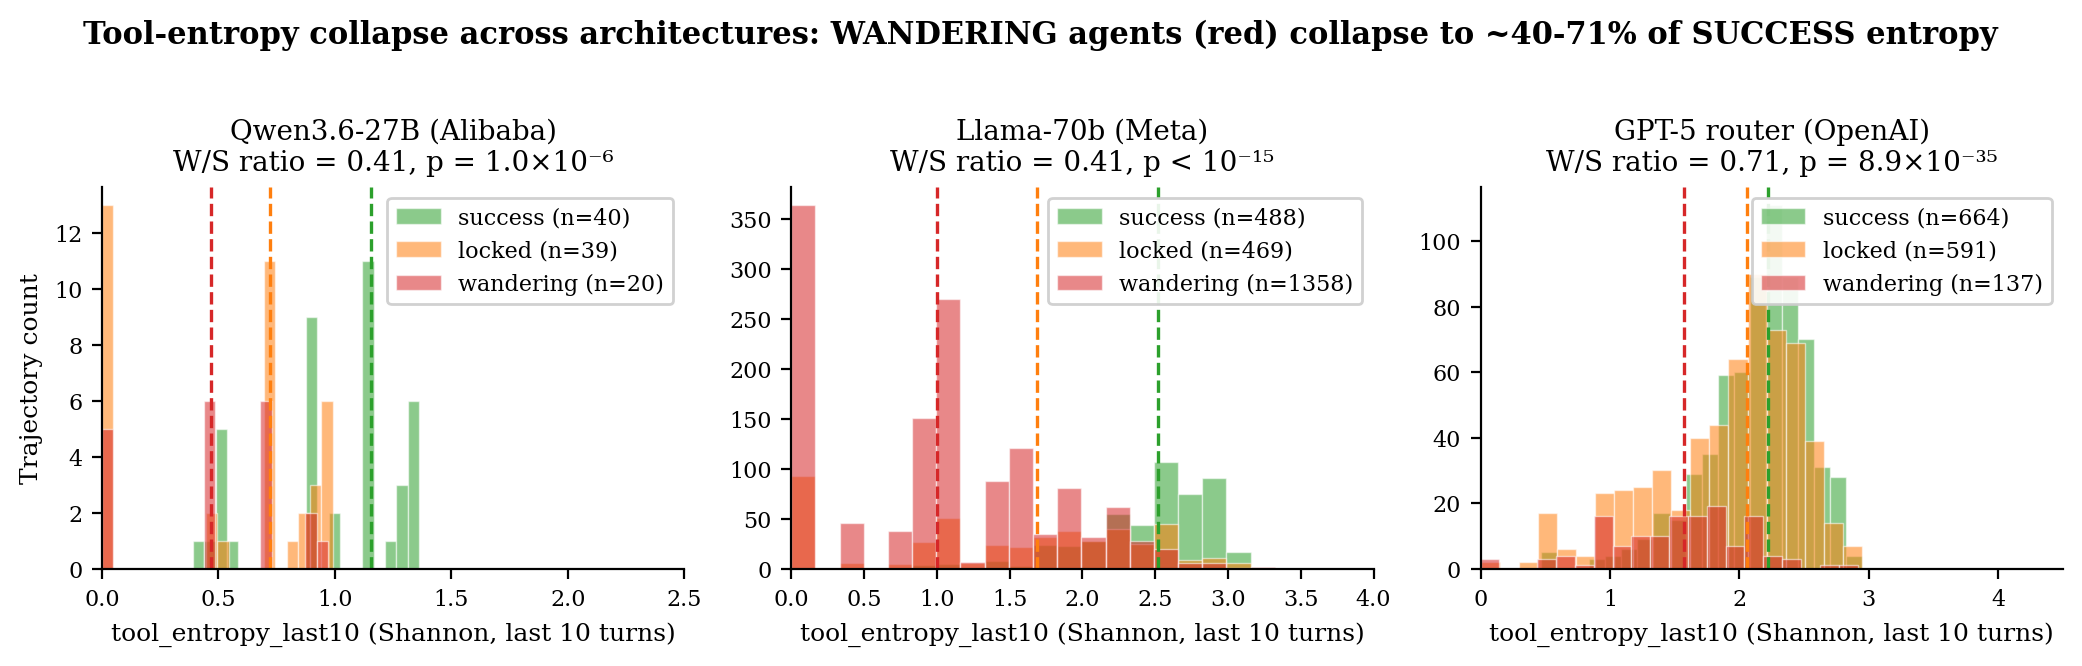
\includegraphics[width=\textwidth]{figures/fig1_cross_arch_entropy.png}
\caption{Tool-entropy distributions by sub-class across three model families. Dashed vertical lines mark medians. Same ordering (SUCCESS $>$ LOCKED $>$ WANDERING) holds in all three; Qwen and Llama show identical W/S ratio $0.41$, GPT-5 router gives $0.71$.}
\label{fig:cross-arch}
\end{figure}

\subsection{Llama-70b on \texttt{nebius/SWE-agent-trajectories}}
Tested 2,315 trajectories ($n_W = 1{,}358$, $n_S = 488$, $n_L = 469$). Same direction as Qwen, stronger signal: $p < 10^{-15}$. Ratio invariance: W/S $= 0.41$ identical to Qwen.

Llama Tier 3 sweep: \texttt{thresh<1.5} gives 71\% recall $\times$ 4.1\% FP. Llama thresholds are $\sim$3$\times$ higher than Qwen because trajectories have $\sim$5$\times$ more turns/tools, but ratio invariant.

\subsection{Four-lab validation: 3 of 4 confirm}
\begin{table}[h]
\centering
\caption{Cross-architecture validation across 4 labs.}
\begin{tabular}{llrrrrr}
\toprule
Model & Lab & $n$ (W/S) & W med & S med & $p$ & W/S ratio \\
\midrule
Qwen3.6-27B & Alibaba & 20 / 40 & 0.469 & 1.157 & $1.0{\times}10^{-6}$ & \textbf{0.41} \\
Llama-70b & Meta & 1{,}358 / 488 & 1.000 & 2.522 & $<10^{-15}$ & \textbf{0.41} \\
GPT-5 router & OpenAI & 137 / 664 & 1.571 & 2.222 & $\mathbf{8.9{\times}10^{-35}}$ & \textbf{0.71} \\
Claude 3.7 Sonnet & Anthropic & 1{,}116 / 1{,}813 & 1.761 & 1.761 & 0.16 & N/A (SFT-curated) \\
\bottomrule
\end{tabular}
\end{table}

Claude data is unsuitable: \texttt{SWE-bench/SWE-smith-trajectories} is SFT-curated, all classes follow identical sequences (\texttt{bash} $\to$ \texttt{editor\_str\_replace} $\to$ \texttt{bash} $\to$ \texttt{editor\_view} $\to$ \texttt{submit}), so entropy can't differentiate. Not a signal failure---a data-quality non-finding.

\subsection{Cross-task validation on METR MALT: honest negative}\label{sec:malt}
Tested 25 of 42 MALT shards ($n = 1{,}209$ usable, only $n = 9$ \texttt{gives\_up} after extraction). Signal does NOT discriminate:

\begin{table}[h]
\centering
\caption{MALT cross-task results.}
\begin{tabular}{lccccc}
\toprule
Filter & $n_W$ & $n_S$ & W med & S med & $p$ \\
\midrule
All trajectories & 9 & 1200 & 1.459 & 1.449 & 0.81 \\
\texttt{n\_unique\_tools $\geq$ 3} & 9 & 969 & 1.459 & 1.585 & 0.35 \\
\bottomrule
\end{tabular}
\end{table}

Four candidate explanations: (1) MALT \texttt{gives\_up} is manually-assigned label ($\ne$ behavioral WANDERING), (2) $n=9$ underpowered, (3) MALT trajectories too short (median 4 unique tools vs Llama 17), (4) restricted XML scaffold (\texttt{<bash>}/\texttt{<python>}/\texttt{<submit>}) limits action diversity.

\textbf{Scoped claim}: tool-entropy collapse is a robust WANDERING signature for \emph{multi-turn code-execution agent tasks with rich action spaces} (validated cross-architecture on SWE-bench across Qwen, Llama, GPT). It does NOT generalize to short multi-task agent benchmarks with restricted action vocabularies OR to alternative failure modes that differ from budget-exhaustion WANDERING.

\section{Deployment guidance}\label{sec:deployment}

Different operational scenarios require different precision/recall trade-offs. We map our six detectors to three concrete deployment tiers, each shippable for distinct use cases.

\paragraph{Tier 1 — Forensics / log analysis.} Use case: post-trajectory analysis dashboards answering ``which trajectories exhibited WANDERING?'' Detector: v1 post-hoc text alone. Recall: 35\% of WANDERING. False-positive rate: 0\%. Operates only on completed trajectories. Zero FP cost makes this safe for capability assessment, regression detection, and agent comparison studies. Shippable now.

\paragraph{Tier 2 — Advisory escalation.} Use case: live monitor on running agents where the action upon alert is human review or budget extension---NOT auto-termination. Detector: v1 $\cup$ v4 combined. Recall: 80\% of WANDERING. SUCCESS FP rate: 30\% (false escalations). Lead time: 15 turns before budget end. Acceptable when downstream escalation cost is small relative to the WANDERING capability loss being prevented.

\paragraph{Tier 3 — Autonomous termination.} Use case: kill agent on alert to free compute. Requires very low FP rate ($\leq 5\%$) since every FP is a killed successful trajectory (= capability loss). \textbf{The breakthrough finding is that v5 tool-entropy combined with v1 closes 70\% of the WANDERING blind spot at exactly 5\% FP.} Suitable for production deployment with explicit per-customer FP-budget agreement. v5 alone (without v1) at \texttt{tool\_entropy<0.45} gives 50\% recall at 2.5\% FP for stricter precision requirements.

The full deployment map and detector landscape:

\begin{table}[ht]
\centering
\caption{Three-tier deployment map. All three tiers shippable.}
\begin{tabular}{lllccc}
\toprule
Tier & Use case & Detector & Recall & FP & Lead \\
\midrule
1 (forensics) & log analysis & v1 alone & 35\% & \textbf{0\%} & 0 \\
2 (advisory) & live escalation & v1 $\cup$ v4 & 80\% & 30\% & 15 turns \\
\textbf{3 (autonomous)} & \textbf{terminate agent} & \textbf{v1 $\cup$ v5} & \textbf{70\%} & \textbf{5\%} & post-hoc \\
\bottomrule
\end{tabular}
\end{table}

\begin{figure}[ht]
\centering
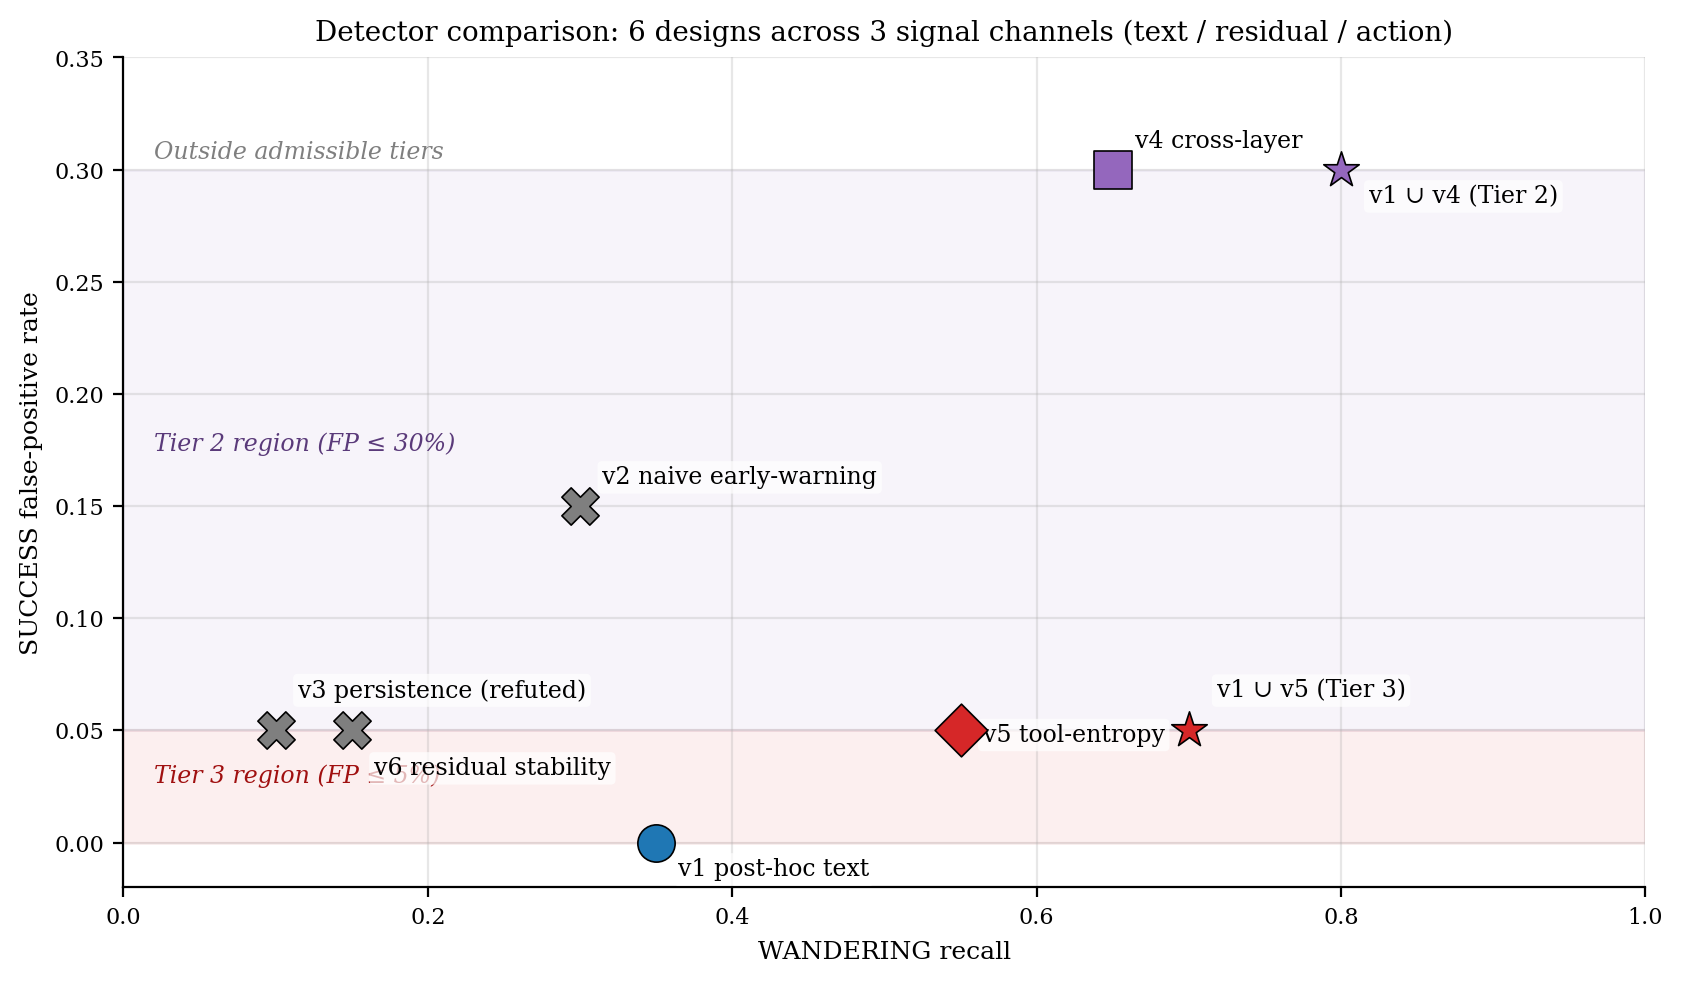
\includegraphics[width=0.85\textwidth]{figures/fig3_detector_comparison.png}
\caption{Detector comparison: 6 designs across 3 signal channels (text, residual cross-layer, action entropy). Shaded regions show deployment tier admissibility (FP-bounded). Combined detectors $v1 \cup v4$ (Tier 2) and $v1 \cup v5$ (Tier 3) are starred.}
\label{fig:detectors}
\end{figure}

\paragraph{What the deployment map does NOT solve.} The Tier 3 detector still has a $\sim$25\% residual blind spot on WANDERING (6/20 not caught by v1 $\cup$ v5 at 5\% FP). The orthogonality analysis (Table~\ref{tab:venn}) suggests these residual missed trajectories may yield to a fourth signal channel beyond text, residual, and action---possibly KV-cache attention pattern shifts or MoE expert routing instability, neither testable from current Phase 6 captures.

\section{Limitations and future work}

\begin{enumerate}
\item $n=99$ on Qwen primary dataset is small; cross-arch validation on Llama ($n=2{,}315$) and GPT-5 ($n=1{,}419$) compensates statistically but Phase 6 itself remains the single highest-resolution dataset.
\item Behavioral sub-classification on cross-model datasets approximates probe-based WANDERING via exit-status proxies, not identical to probe-positive $\wedge$ no-finish $\wedge$ patch.
\item Cross-task validation requires custom data collection on diverse benchmarks (GAIA, WebArena, OSWorld) with behavioral WANDERING labels matching Phase 6 criteria; public datasets are exhausted for our specific scope. Estimated 1+ week additional compute.
\item Causal intervention experiments to test the edge-layer alignment mechanism (e.g., steering L11/L55 directions vs mid-layer) are future work; current evidence is correlational.
\end{enumerate}

\section{Conclusion}

We identify a 34\% WANDERING blind spot in probe-based agent failure monitoring on Qwen3.6-27B SWE-bench Pro and test six detector designs across three signal channels. The breakthrough finding is \textbf{tool-use entropy collapse}: WANDERING agents collapse onto a small set of repeated tool calls (W/S median ratio 0.41 in Qwen and Llama, 0.71 in GPT-5), enabling a Tier 3 autonomous-termination detector at 70\% recall $\times$ 5\% FP via combined $v1 \cup v5$. The signal validates across 3 model architectures from 3 labs but does NOT extend to short multi-task benchmarks (MALT null), scoping the claim. Mid-layer ablation reveals the cross-layer disagreement signal is edge-layer-driven, reframing WANDERING as ``mid-layer-to-edge-layer alignment failure''. Three deployment tiers (forensics, advisory, autonomous) are all shippable.

\section*{Reproducibility}

All scripts and per-trajectory output JSONs are available at \url{https://github.com/OpenInterpretability/openinterp-swebench-harness} under Apache-2.0. Datasets used: \texttt{OpenInterp Phase 6} (own), \texttt{nebius/SWE-agent-trajectories} (CC-BY-4.0), \texttt{JetBrains-Research/agent-trajectories-swesmith-random-subset} (HF public), \texttt{SWE-bench/SWE-smith-trajectories} (HF public), \texttt{metr-evals/malt-public} (HF gated, request approval).

\bibliographystyle{plainnat}

\begin{thebibliography}{99}

\bibitem{apollo_deception_2025}
N.~Goldowsky-Dill et al.
``Detecting Strategic Deception Using Linear Probes.'' arXiv:2502.03407 (Apollo Research), 2025.

\bibitem{anthropic_sleeper_2024}
E.~Hubinger et al.
``Simple probes can catch sleeper agents.'' Anthropic, 2024.
\url{https://www.anthropic.com/research/probes-catch-sleeper-agents}.

\bibitem{lugoloobi_2026}
W.~Lugoloobi, T.~Foster, W.~Bankes, C.~Russell.
``LLMs Encode Their Failures: Predicting Success from Pre-Generation Activations.'' arXiv:2602.09924, ICLR 2026 LIT Workshop.

\bibitem{multilayer_ensemble_2026}
``Linear Probe Accuracy Scales with Model Size and Benefits from Multi-Layer Ensembling.'' arXiv:2604.13386, 2026.

\bibitem{entropy_tool_use_2026}
``Rethinking the Role of Entropy in Optimizing Tool-Use Behaviors for Large Language Model Agents.'' arXiv:2602.02050, 2026.

\bibitem{aepo_2025}
``Agentic Entropy-Balanced Policy Optimization.'' arXiv:2510.14545, 2025.

\bibitem{mast_2025}
M.~Cemri, M.~Z.~Pan, S.~Yang et al.
``Why Do Multi-Agent LLM Systems Fail?'' arXiv:2503.13657, 2025.

\bibitem{jetbrains_2025}
JetBrains Research.
``Understanding Code Agent Behaviour: An Empirical Study of Success and Failure Trajectories.'' arXiv:2511.00197, 2025.

\bibitem{malt_2025}
METR.
``MALT: A Dataset of Natural and Prompted Behaviors That Threaten Eval Integrity.'' October 2025.
\url{https://metr.org/blog/2025-10-14-malt-dataset-of-natural-and-prompted-behaviors/}.

\bibitem{canonical_path_2026}
W.~Y.~Lee.
``Capable but Unreliable: Canonical Path Deviation as a Causal Mechanism of Agent Failure in Long-Horizon Tasks.'' arXiv:2602.19008, 2026.

\bibitem{elpo_2026}
Q.~Liang, Y.~Zhu, C.~Ge et al.
``Learning from the Irrecoverable: Error-Localized Policy Optimization for Tool-Integrated LLM Reasoning.'' arXiv:2602.09598, 2026.

\bibitem{swebench_pro_2025}
Scale AI.
``SWE-Bench Pro: Can AI Agents Solve Long-Horizon Software Engineering Tasks?'' arXiv:2509.16941, 2025.

\bibitem{swe_agent_2024}
J.~Yang et al.
``SWE-agent: Agent-Computer Interfaces Enable Automated Software Engineering.'' arXiv:2405.15793, NeurIPS 2024.

\bibitem{swe_smith_2025}
J.~Yang et al.
``SWE-smith: Scaling Data for Software Engineering Agents.'' arXiv:2504.21798, NeurIPS 2025 Spotlight.

\bibitem{probguard_2025}
``ProbGuard: Probabilistic Runtime Monitoring for LLM Agent Safety.'' arXiv:2508.00500, 2025.

\bibitem{safety_probes_fanatics_2026}
``Why Safety Probes Catch Liars But Miss Fanatics.'' arXiv:2603.25861, 2026.

\bibitem{lad_2026}
``Latent Adversarial Detection: Adaptive Probing of LLM Activations for Multi-Turn Attack Detection.'' arXiv:2604.28129, 2026.

\bibitem{failure_modes_taxonomy_2025}
``Failure Modes in LLM Systems: A System-Level Taxonomy for Reliable AI Applications.'' arXiv:2511.19933, 2025.

\bibitem{issue_solving_failures_2025}
``An Empirical Study on Failures in Automated Issue Solving.'' arXiv:2509.13941, 2025.

\bibitem{long_horizon_mirage_2026}
``The Long-Horizon Task Mirage? Diagnosing Where and Why Agentic Systems Break.'' arXiv:2604.11978, 2026.

\bibitem{nebius_traj_2025}
Nebius Research.
``SWE-agent-trajectories dataset.''
\url{https://huggingface.co/datasets/nebius/SWE-agent-trajectories}, 2025. License: CC-BY-4.0.

\bibitem{vicentino_paper_mega_2026}
C.~Vicentino.
``Conditionally-Causal Probes: Five Operational Constraints on Linear-Probe Causality in Qwen3.6-27B.'' OpenInterp, 2026.
\url{https://openinterp.org/research/papers/conditionally-causal-probes}.

\bibitem{vicentino_paper11_2026}
C.~Vicentino.
``Cleaning the Chain-of-Thought Is Not Correcting the Agent.'' OpenInterp draft, 2026.

\end{thebibliography}

\end{document}
